\documentclass[8pt, xcolor = dvipsnames]{beamer}



\usepackage{beamerthemesplit}
\renewcommand{\baselinestretch}{1.5}\normalsize % Zeilenabstand 1.5
\usepackage{caption}
\makeatletter
\newcommand\notsotiny{\@setfontsize\notsotiny{7}{7}}

\newcommand\middletiny{\@setfontsize\notsotiny{6}{6}}
\makeatother
\usepackage{numprint}
\npthousandsep{\,}
\usepackage{csquotes}
\usepackage{array}
\usepackage{dirtytalk}
\usepackage{amsmath}
\usepackage{bm}
\usepackage{multirow}
\usepackage{amssymb}
\usepackage{amsthm}
\usepackage{amsfonts}
\usepackage{color}
\usepackage{layouts}
% printing the textsize used
% \printinunitsof{cm}
% \prntlen{\textwidth}
\usepackage{tabularx}
\usepackage{graphicx}
\usepackage{pdfpages}
\usepackage[ngerman]{babel}

%\usetheme{default}
%\usetheme{AnnArbor}
%\usetheme{Antibes}
%\usetheme{Bergen}
%\usetheme{Berkeley}
\usetheme{Berlin}
%\usetheme{Boadilla}
%\usetheme{CambridgeUS}
%\usetheme{Copenhagen}
%\usetheme{Darmstadt}
%\usetheme{Dresden}
%\usetheme{Frankfurt}
%\usetheme{Goettingen}
%\usetheme{Hannover}
%\usetheme{Ilmenau}
%\usetheme{JuanLesPins}
%\usetheme{Luebeck}
%\usetheme{Madrid}
%\usetheme{Malmoe}
%\usetheme{Marburg}
%\usetheme{Montpellier}
%\usetheme{PaloAlto}
%\usetheme{Pittsburgh}
%\usetheme{Rochester}
%\usetheme{Singapore}
%\usetheme{Szeged}
%\usetheme{Warsaw}
%\usecolortheme[named=RoyalBlue]{structure}
\usecolortheme{seahorse}

\usepackage{listings}


\usepackage[T1]{fontenc}          % erlaubt Umlaute (Zeichenbelegung)
\usepackage[utf8x]{inputenc}     % erlaubt �-Eingabe �ber die Tastatur
\usepackage[ngerman]{babel}  
\usepackage{amsmath,amsfonts,amssymb}

\usepackage{xcolor}

%%%%%%%%%%%%%%%Foliennummerierung%%%%%%%%%%%%%%%%%%%%%%%%%%%%%%%%%%%%%%%%%
\setcounter{framenumber}{0} 
\setbeamertemplate{footline}[frame number]
%%%%%%%%%%%%%%%Foliennummerierung%%%%%%%%%%%%%%%%%%%%%%%%%%%%%%%%%%%%%%%%%

\title{\textit{Multiclass}-Klassifizierung \\
 von Nachrichten Schlagzeilen}        % Titel (Kommando muss aufgerufen werden)
\author{Marc Schmieder}     % Autor(en) 
\date{06.02.2020}

\subtitle{Vergleich zwischen neuronalen Netzen und baumbasierten Algorithmen auf verschiedenen Repräsentationen von Wörtern}  % etwas kleinere Schrift als der Titel
\institute{Prof. Dr. Andreas Groll, Statistical Methods for Big Data, TU Dortmund} % Betreuer/Uni/Veranstaltung/etc.


\begin{document}                  % Ende der Pr�ambel, Beginn der Pr�sentation

\begin{frame}                     % Titelfolie
 \maketitle                       % Kommando zum Aufruf der Titelfolie
\end{frame}

%%%%%%%%Beginn%%%%%%%%%%%%%%%%%%%%%%%%%%


\tableofcontents

\section{Motivation und Zielstellung}
\begin{frame}

   \begin{itemize}
   \item 
   \end{itemize}
\end{frame}  


\section{Datensatz und Exploration}


\begin{frame}{Datensatz I}

   \begin{itemize}
   \item \textit{News Category Dataset} von Machine Learning Plattform \textit{Kaggle}, Sprache: Englisch
   \item \numprint{200853} Beobachtungen, mit Informationen  über Artikel der US-Amerikanischen Onlinezeitung \textit{Huffpost}
   \item  Veröffentlichungszeitraum: 28.01.2012 bis zum 25.05.2018 (> $6$ Jahre)
   \item Spalten: Schlagzeile, Author(en), Link zum Artikel, Kurzbeschreibung, Datum, Kategorie
   \item Kategorie ist Zielvariable ($41$ Ausprägungen), unabhängige Variable ist nur die Schlagzeile
   \end{itemize}

\end{frame}


\begin{frame}{Datensatz II}

\begin{table}[ht]
\centering
\notsotiny
\begin{tabular}{|m{1cm}||lll|}
  
  \hline
Daten\-punkt & Kategorie & Schlagzeile & Author(en)  \\ 
  \hline
1 & STYLE \& BEAUTY & Kardashians Eyewear: \dots  & Jessica Misener \\  
2 &  WELLNESS & Sports Drink Alternatives? 7  \dots & Meredith Melnick \\
3 &  STYLE \& BEAUTY & Nicole Kidman's Topless \dots & Ellie Krupnick \\
4 &  SCIENCE & Second Man On Moon Claims  \dots & Tyler McCarthy \\
5 &  ENTERTAINMENT & Popcorn Preview: House of  (2013) & Leslie Sisman \dots \\

   \hline
   \hline
Daten\-punkt & Link & Kurzbeschreibung & Datum \\
   \hline
1 & https://www.huffing \dots & What else can we photoshop \dots & 2012-08-10 \\   2 & https://www.huffing \dots & In this scenario, homemade, all \dots & 2012-06-04 \\ 
3 & https://www.huffing \dots & PHOTOS: From the very first \dots & 2014-01-10 \\ 
4 & https://www.huffing \dots & - & 2014-04-29 \\ 
5 & https://www.huffing \dots & House of Cards is a smart, s\dots & 2013-03-31 \\ 
\hline 

\end{tabular}

\caption{Ausschnitt von 4 Datenpunkten aus dem unbearbeiteten Datensatz}
\end{table}

\end{frame}  



 \subsection{Veränderung am Datensatz}

\begin{frame}{Cleaning}
\begin{itemize}
   \item Konvertierung der Großbuchstaben zu Kleinbuchstaben (\textit{Teacher}, \textit{teacher})
   \item Ursprung aus verschiedenen Ländern: Entfernung von Sonderzeichen (\say{©} oder \say{™}), da Konvertierungsfehler
   \item  \say{n't} $\xrightarrow{}$ \say{ not}, \say{'ll} $\xrightarrow{}$ \say{ will},  \say{here's} $\xrightarrow{}$ \say{here is} 
   \item \say{trump's} $\xrightarrow{}$ \say{trump his}, dann \say{john's son} $\xrightarrow{}$ \say{john its son}
   \item Entfernung von leeren Texten (6 Beobachtungen). Insgesamt \numprint{200847} Beobachtungen verbleibend.
   \end{itemize}
\end{frame}



\begin{frame}{Zusammenlegung der Kategorien I}

   \begin{itemize}
   \item Namentliche und inhaltliche Ähnlichkeit der Kategorien (\textit{arts \& culture} und \textit{culture & arts})
   \item Schwierig mit menschlicher Intuition auseinander zu halten.
   \item Reduktion auf $32$ Kategorien (ab $0.50$, zuzüglich \textit{arts \& culture} \textit{arts})
   \end{itemize}
 
 \begin{table}[ht]
\begin{center}
\notsotiny
\begin{tabular}{ | p{0.1 \textwidth} | p{0.42 \textwidth}| p{0.42 \textwidth} | }
  \hline
Beispiel & Kategorie \textit{parents}  & Kategorie \textit{parenting} \\ 
  \hline
1 & 40 tweets that sum up life with 4-year-olds & a baby book of disasters \\ 
  2 & these were the trendiest baby names in the late '80s & it is time to find your tribe \\ 
  3 & these quotes from kids are hilarious, adorable and oddly insightful & help huffpost parents win a webby award! \\ 
  4 & 30  'star wars'-inspired names parents are giving their babies & why our 'imperfect' moments are perfect to our children \\ 
   \hline
\end{tabular}
\caption{Beispiele für Schlagzeilen der Kategorien \textit{parents} und \textit{parenting}}
\label{tab:parentsMerge}
\end{center}
\end{table}
 
\end{frame}
 
 
\begin{frame}{Zusammenlegung der Kategorien II}

\begin{table}[ht]
\begin{center}
\notsotiny
\begin{tabular}{|l|l|c|c|}

  \hline
Kategorie 1 & Kategorie 2  & relative Schnittmenge & neue Kategorie\\
  \hline
\textit{healthy living} & \textit{wellness} & 0.76 & \textit{wellness \& healthy living} \\ 
  \textit{parents} & \textit{parenting} & 0.74 & \textit{parents} \\ 
  \textit{taste} & \textit{food \& drink} & 0.70 & \textit{food, drink \& taste}\\ 
   \vdots & \vdots & \vdots & -\\
  \textit{fifty} & \textit{parenting} & 0.50 & -\\ 
    \vdots & \vdots & \vdots & -\\
  \textit{parents} & \textit{fifty} & 0.48 & - \\ 
  \textit{arts \& culture} & \textit{arts} & 0.46 & \textit{arts \& culture}\\  
  \vdots & \vdots & \vdots & -\\

  \textit{crime} & \textit{food \& drink} & 0.04 & -\\
  \hline 
  \hline 
  \multicolumn{2}{|c|}{Mittelwert} &  0.24 & \\
   \hline
\end{tabular}
\caption{Relative Schittmenge der $100$ häufigsten Wörter für Paare an Kategorien}
\label{tab:categoryMerge}
\end{center}
\end{table}
   
\end{frame}   







\begin{frame}{\insertsection}

   \begin{itemize}
   \item 
   \end{itemize}
 
   
\end{frame}   




\begin{frame}

\begin{figure}[ht]
    \centering
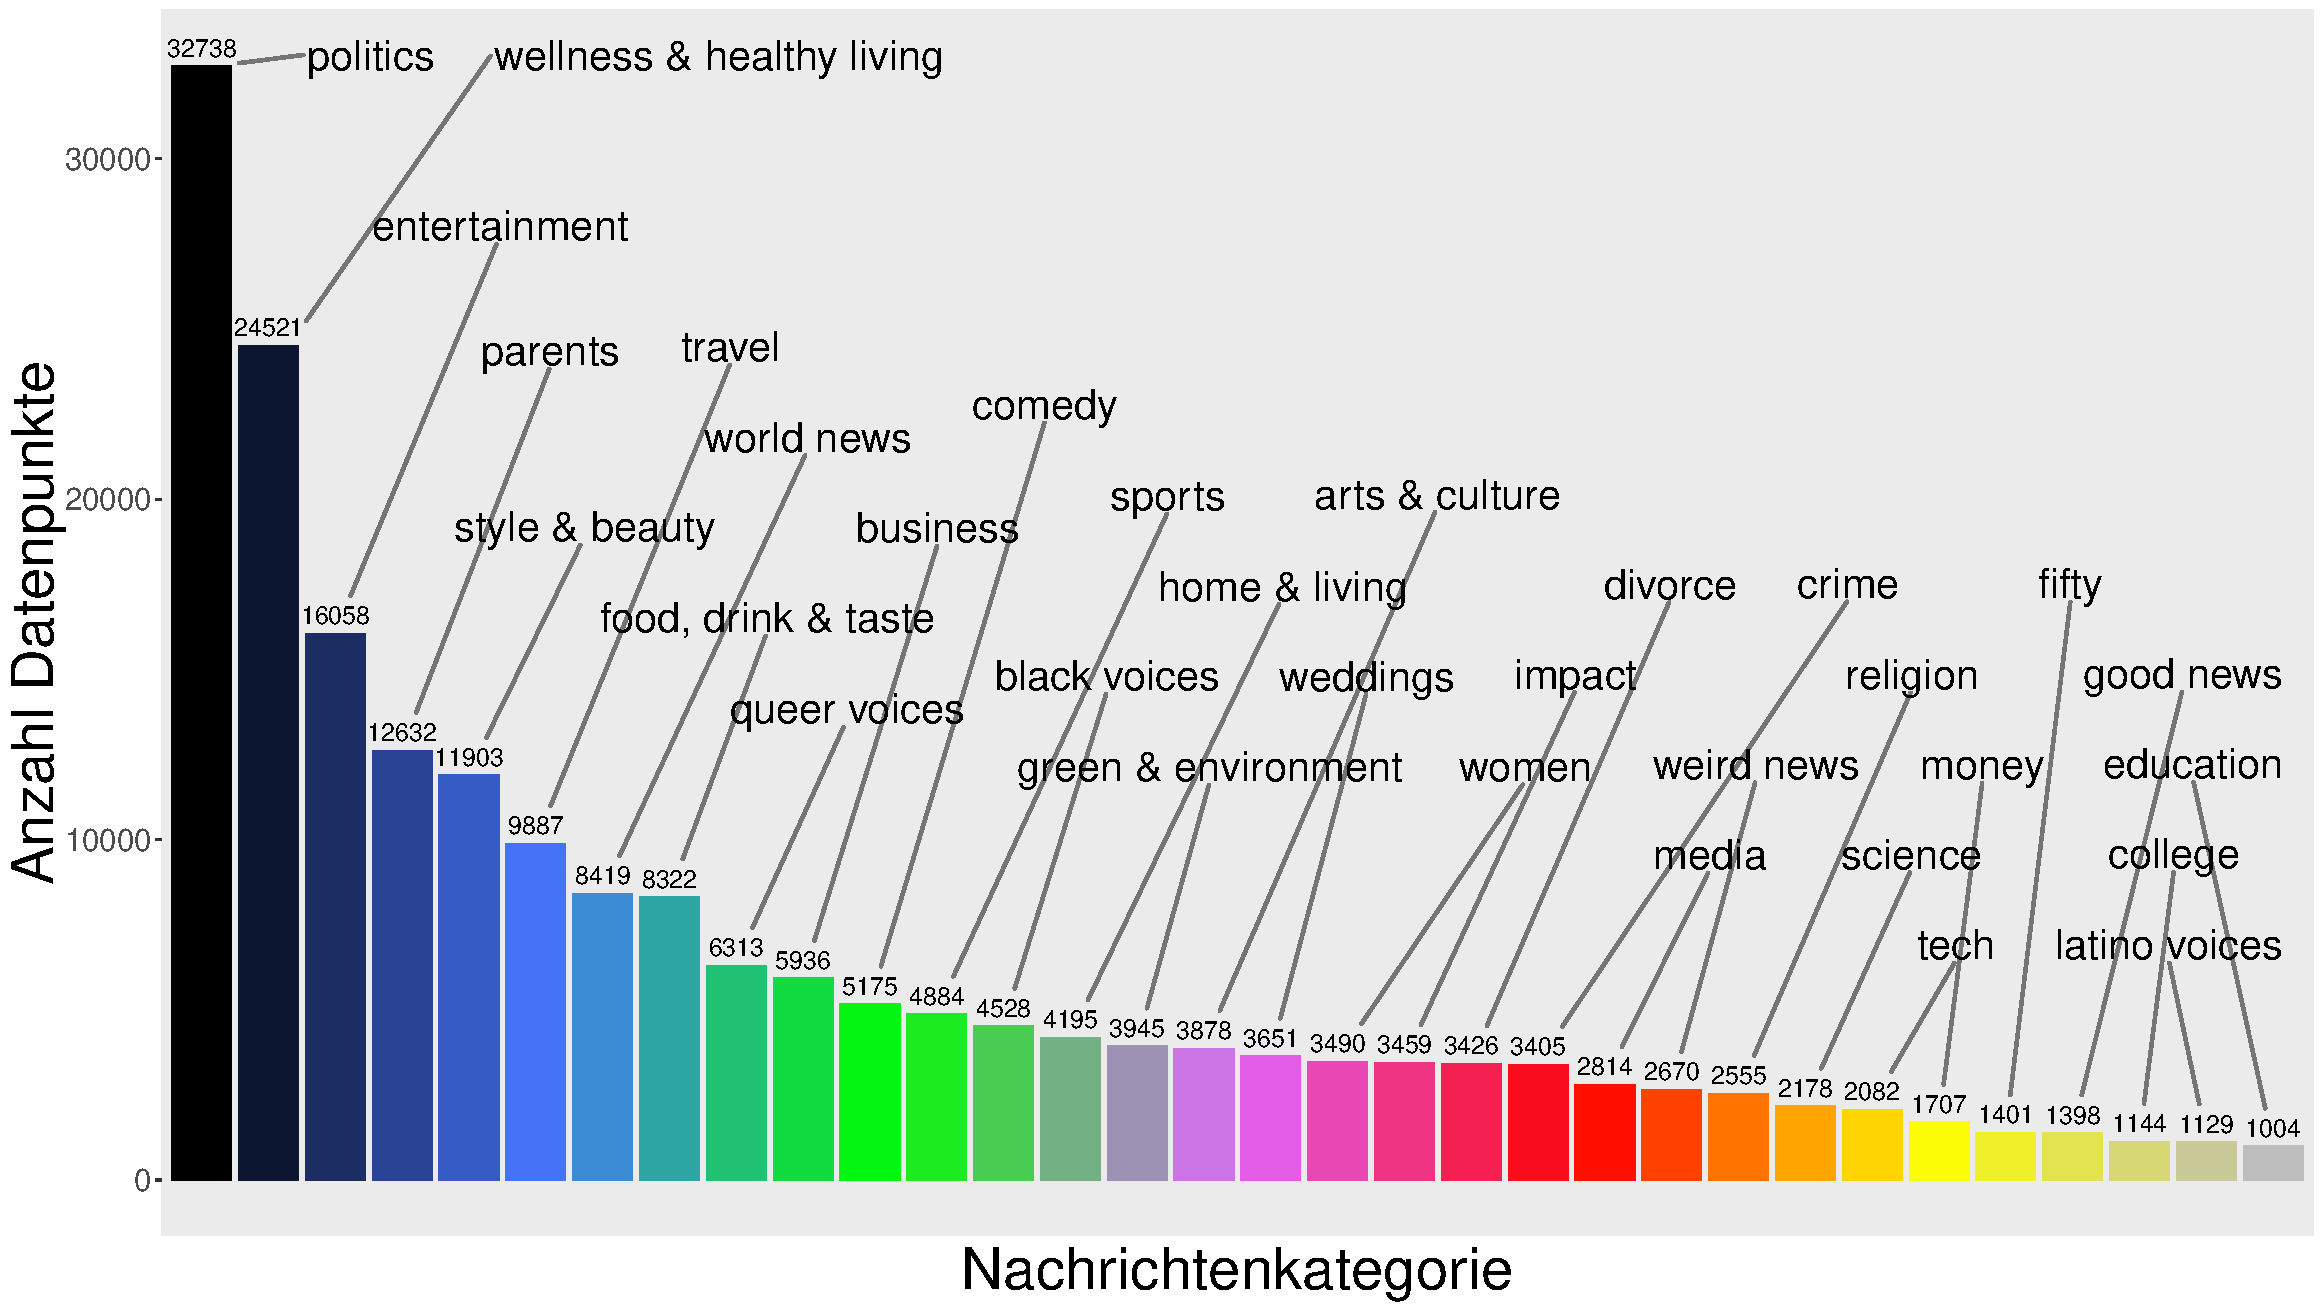
\includegraphics[width = \textwidth,  keepaspectratio]{Images/barplotCategories.pdf} 
\caption{Anzahl Datenpunkte pro Nachrichtenkategorie}
\label{abb:barplotCategories}
\end{figure}

\end{frame}


\begin{frame}

\begin{figure}[ht]
    \centering
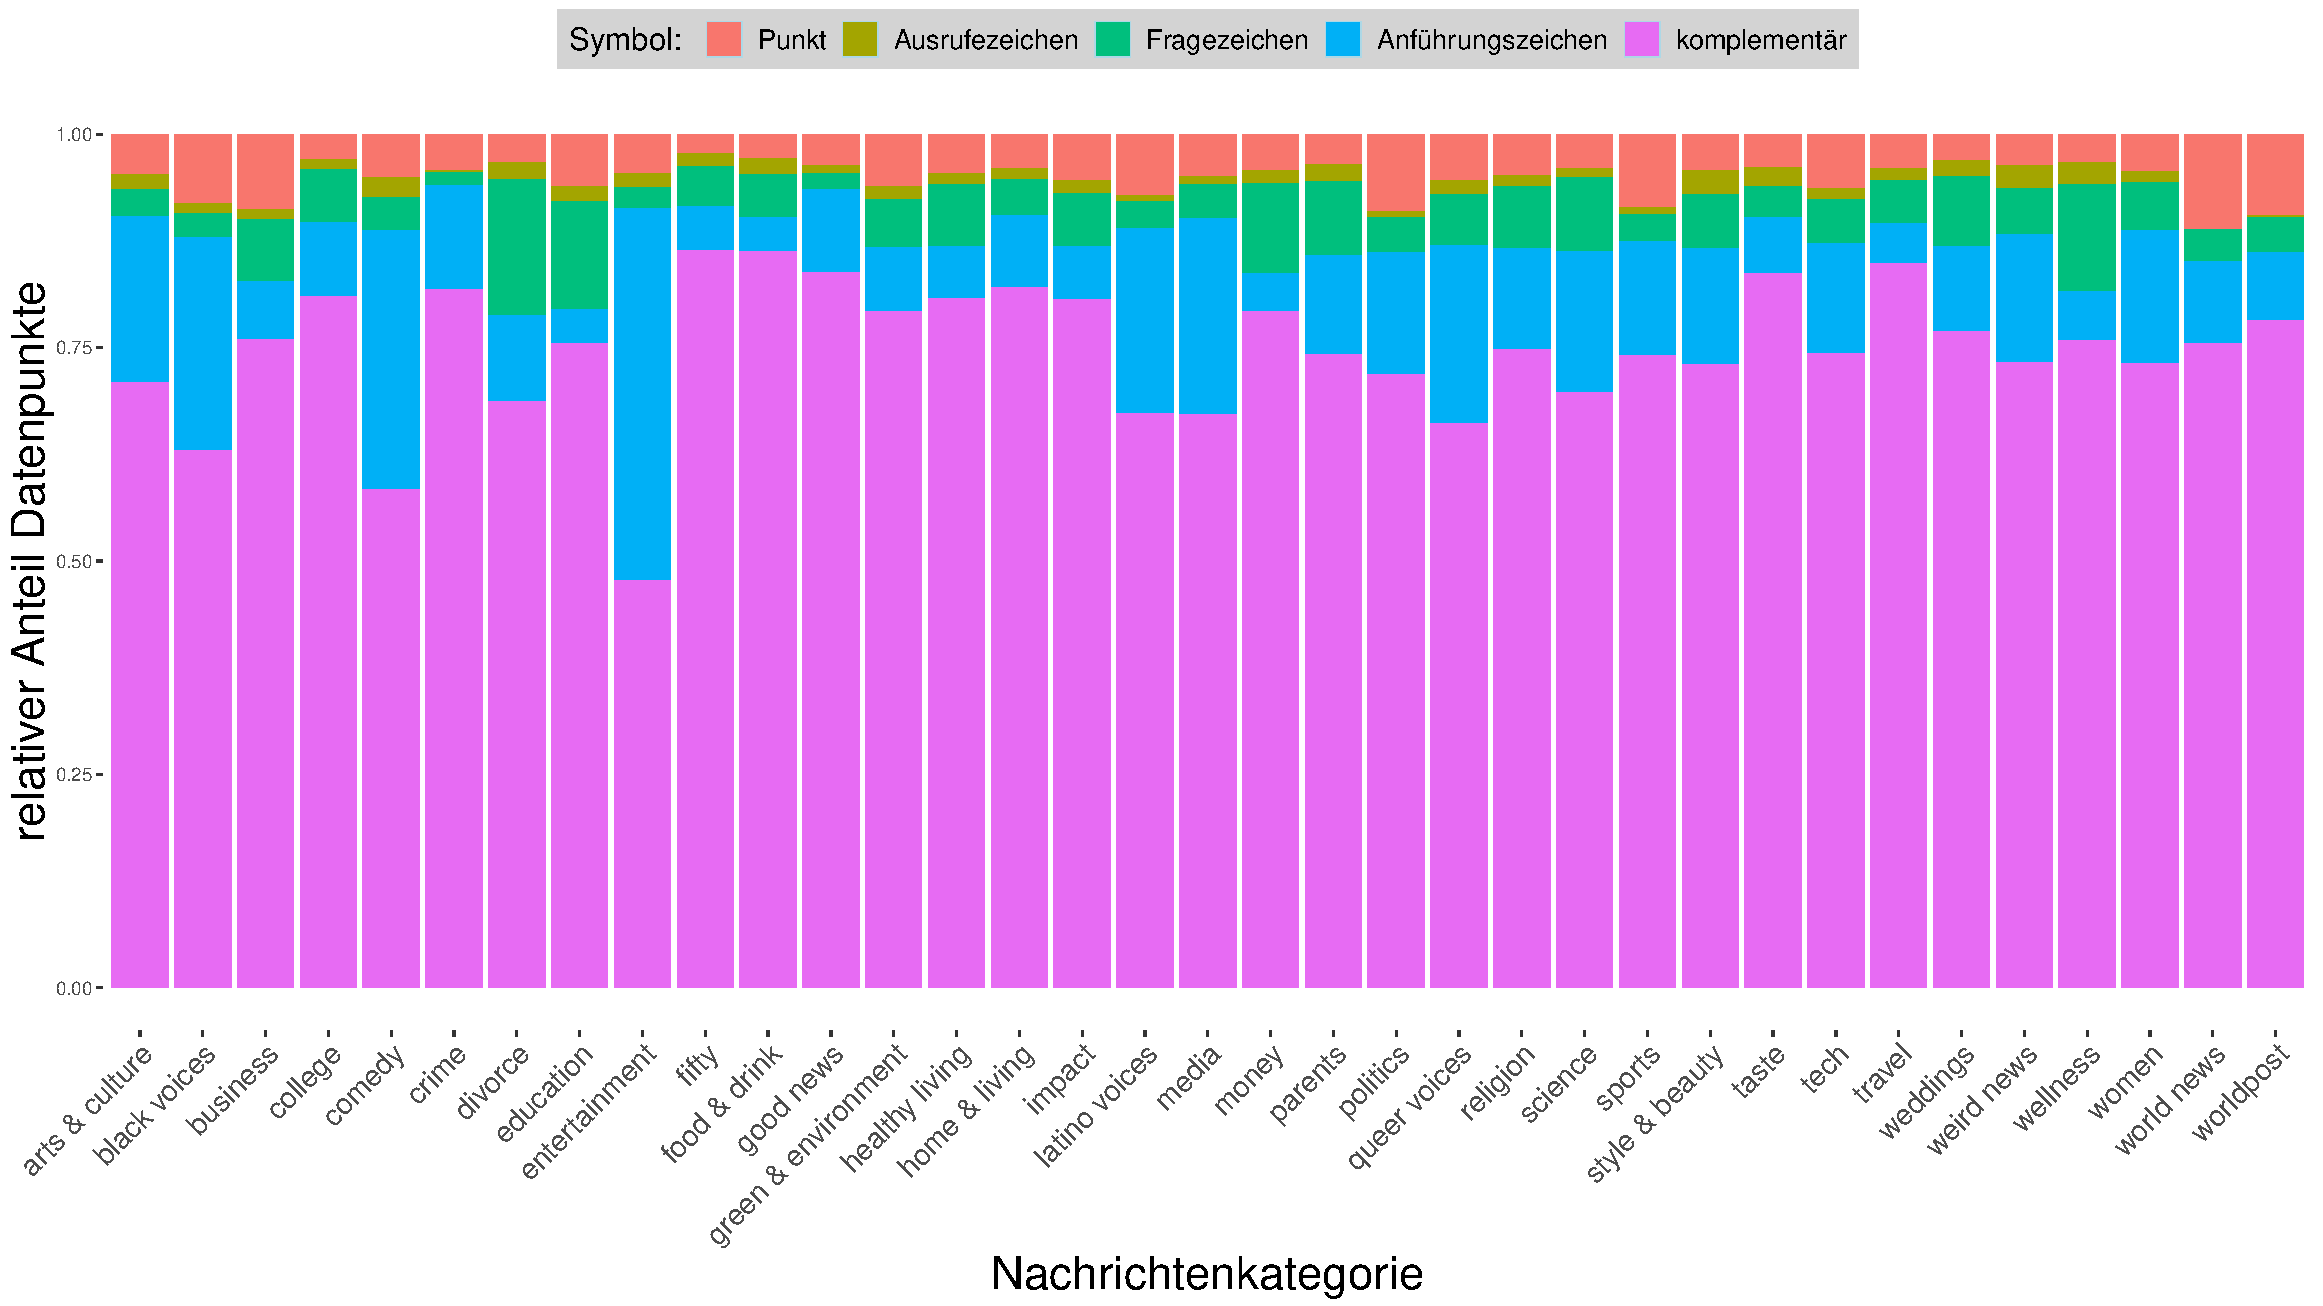
\includegraphics[width = \textwidth,  keepaspectratio]{Images/barplotSymbols.pdf} 
\caption{Relativer Anteil Datenpunkte für ausgewählte Sonderzeichen pro Kategorie. Der komplementäre Anteil ist der Anteil Datenpunkte, in dem keine der aufgeführten Sonderzeichen enthalten sind.}
\label{abb:barplotSymbols}
\end{figure}

\end{frame}


\begin{frame}
\begin{figure}[ht]
    \centering
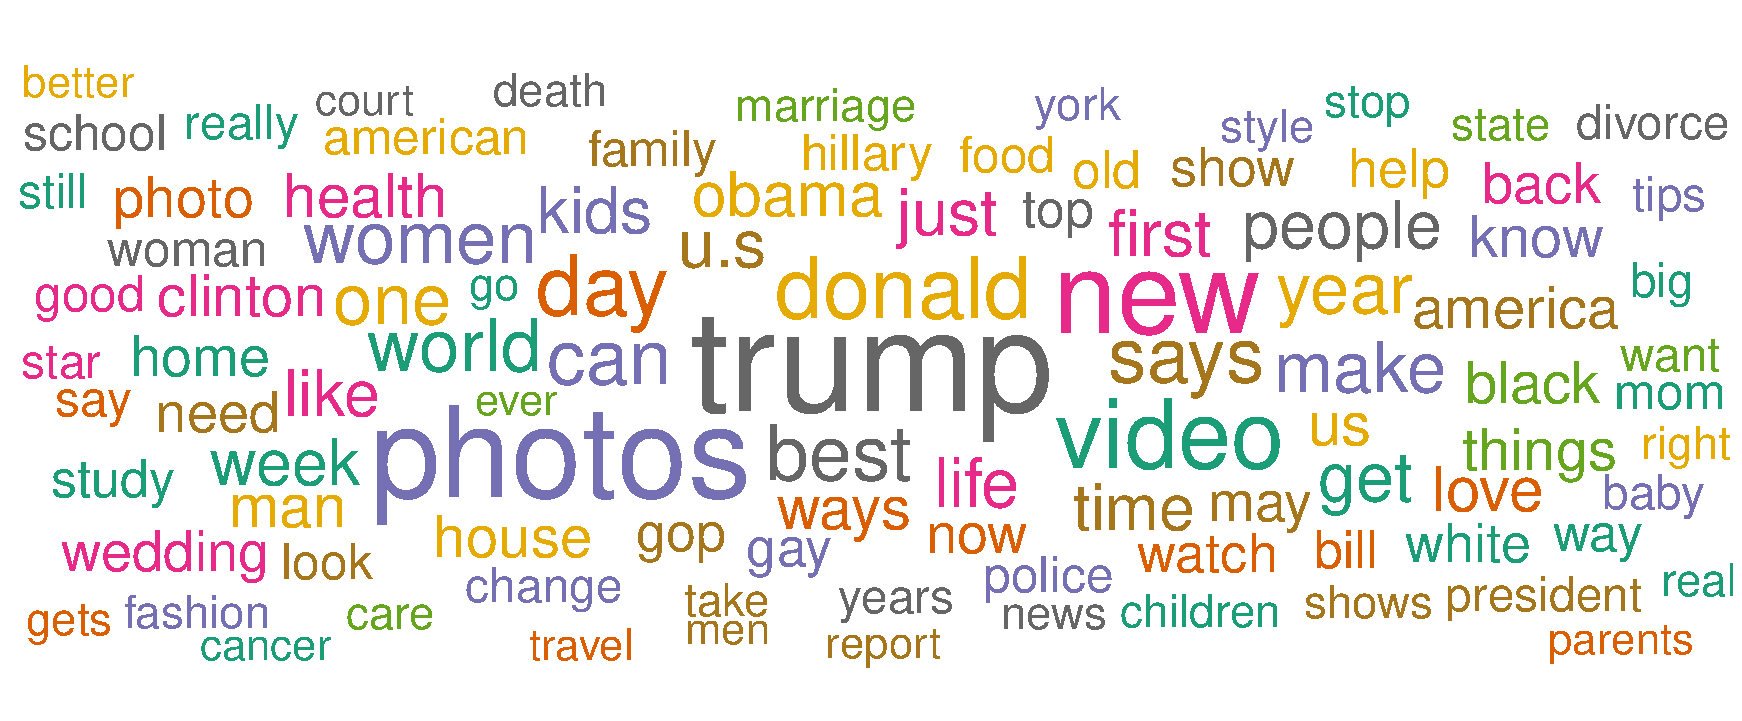
\includegraphics[width = \textwidth,  keepaspectratio]{Images/wordCloudAll.pdf} 
\caption{\textit{wordcloud} für die häufigsten 100 Wörter aller Kategorien}
\label{abb:WordcloudAll}
\end{figure}
\end{frame}


\section{Repräsentation der Wörter}



\begin{frame}{Bag-Of-Words}

\begin{table}[ht]
\begin{center}

\begin{tabular}{|c||ccccccccccc|}
\hline
\multicolumn{12}{|c|}{\textit{BOW} \textit{dtm}} \\
\hline 
   Satz   & the & dog & cat & like & likes &  to & sit  & owner & his &  does & not \\
      \hline
Satz 1 & $1$ & $0$ & $1$ & $0$ & $1$ & $1$ & $1$ & $0$ & $0$ &  $0$ & $0$ \\
Satz 2 & $1$ & $1$ & $0$ & $1$ & $0$ & $0$ & $0$ & $1$ & $1$ &  $1$ & $1$ \\
Satz 3 & $0$ & $1$ & $0$ & $0$ & $1$ & $0$ & $0$ & $1$ & $0$ &  $0$ & $0$ \\

\hline

\end{tabular}
\end{center}{}
\caption{Beispiel für eine \textit{document-term-matrix} für die $3$ Beispielsätze \textit{the cat likes to sit}, \textit{the dog does not like his owner}, \textit{the owner likes the dog} jeweils für das \textit{BOW Embedding} und das \textit{TFIDF Embedding} }  
\label{tab:BOWExample}

\end{table}
\end{frame}{}

\begin{frame}{GloVe: Global Word Vektors}


\begin{itemize}
    \item Methode zur Repräsentation von Wörtern im $F$- dimensionalen Raum
    \item Training auf eigenem Textkorpus
    \item Vortrainierte Datensätze auf Wikipedia oder Common Crawl
    \item Datenpunkt ist Sequenz aus Wort Vektoren und hat Matrix-Form mit Dimension $F \times maxWords$
\end{itemize}{}
    
\end{frame}{}


\begin{frame}{GloVe: Global Word Vektors}
    \begin{table}[ht]
    \notsotiny
    \begin{center}
 \begin{tabular}{|l||ccccccccccc|}
  \hline
  & \multicolumn{11}{|c|}{Kontext} \\
\hline 
Wörter & the & dog & cat & like & likes & to & sit & owner & his & does & not \\ 
  \hline
the & 0 & 0 & 0 & 0 & 0 & 0 & 0 & 0 & 0 & 0 & 0 \\ 
  dog & 2  & 0  & 0  & 0  & 1 & 0 & 0 & 0 & 0 & 0 & 0 \\ 
  cat & 1 & 0 & 0 & 0 & 1 & 1 & 0 & 0 & 0 & 0 & 0 \\ 
  like & 0 & 0 & 0 & 0 & 0 & 0 & 0 & 1 & 0 & 0 & 1 \\ 
  likes & 3 & 0 & 0 & 0 & 0 & 0 & 0 & 0 & 0 & 0 & 0 \\ 
  to & 0 & 0 & 0 & 0 & 1 & 0 & 0 & 0 & 0 & 0 & 0 \\ 
  sit & 0 & 0 & 0 & 0 & 1 & 1 & 0 & 0 & 0 & 0 & 0 \\ 
  owner & 2 & 0 & 0 & 0 & 1 & 0 & 0 & 0 & 0 & 0 & 0 \\ 
  his & 0 & 0 & 0 & 1 & 0 & 0 & 0 & 1 & 0 & 0 & 1 \\ 
  does & 1 & 1 & 0 & 1 & 0 & 0 & 0 & 0 & 0 & 0 & 1 \\ 
  not & 0 & 1 & 0 & 0 & 0 & 0 & 0 & 0 & 0 & 0 & 0 \\ 
   \hline
\end{tabular}  
 
\end{center}{}
\caption{Beispiel für eine \textit{term-co-occurance} Matrix für die $3$ Beispielsätze \textit{the cat likes to sit} (Satz $1$), \textit{the dog does not like his owner} (Satz $2$), \textit{the owner likes the dog} (Satz $3$) für einen symmetrischen Fensterbereich von 2}  
\label{tab:GloveExample}

\end{table}
\end{frame}{}




\section{Verfahren}

\begin{frame}{Verfahren}
\begin{itemize}

    \item XGBoost: Baum-Boosting Verfahren
    \item MLP: Multi-Layer Perceptron: Reguläres Feed-forward neuronales Netz
    \item CNN: Convolutional Neural Network
    \item Bi-LSTM: Bidirectional Long-Short-Term-Memory Neural Network
   
\end{itemize}
\end{frame}


\begin{frame}{XGBoost}
    
\end{frame}{}


\begin{frame}{Multi Layer Perceptron}
    
\end{frame}{}

\begin{frame}{Convolutional Neural Net}
    
\begin{figure}[!ht]
\begin{center}
\includegraphics[width = \textwidth,  keepaspectratio]{Images/CNN_NLP.PNG}
\caption{Architektur eines \textit{CNN} für einen NLP Anwendungsfall}
\label{abb:CNN_NLP}
\end{center}
\end{figure}
\end{frame}{}

\begin{frame}{Long-Short-Term-Memory Neural Net}
    \begin{figure}[!ht]
\begin{center}
\includegraphics[width = \textwidth,  keepaspectratio]{Images/RNN_Example_DeepNLPpage128.PNG}
\caption{\textit{RNN} Model bei Input des Satzes: Sachin is a great }
\label{abb:RNNExample}
\end{center}
\end{figure}
\end{frame}{}

\section{Auswertung}

\begin{frame}{Framework}
\begin{itemize}
    \item Einteilung der \numprint{200847} Beobachtungen des gesamten Datensatzes in Trainings-, Test- und Validierungsdaten \item Testdaten $\numprint{20005}$ Beobachtungen, etwa 10 Prozent (Erwartungsgemäß $100$ in der kleinsten Kategorie)
    \item Von den $90$ Prozent der Daten, Stichprobe von $10$ Prozent gezogen ($9$ Prozent der gesamten Daten). $\numprint{18084}$ Beobachtungen
    \item Davon $80$ Prozent Trainingsdaten der Vorauswahl ($\numprint{14467}$ Datenpunkte) und $20$ Prozent  Validierungsdaten der Vorauswahl ($\numprint{3617}$ Datenpunkte)
    \item Tuning und Struktur der Netze auf Validierungsdaten
\end{itemize}{}
\end{frame}{}


\begin{frame}{Finale Auswahl und Evaluation}

\begin{table}[ht]
\notsotiny
\centering
\begin{tabular}{|l||ccccc|}
  \hline
\textit{Embedding}, Modell & $accuracy$ & $\overline{accuracy}$ & $fscore_M^{(1)}$ & $CE$ & $\bar{p}_{IfCorrect}$ \\ 
  \hline
\textit{BOW, XGBoost} & \textcolor{red}{0.624} & 0.487 & 0.541 & \textcolor{red}{1.447} & 0.653 \\ 
  \textit{GloVe 300D, CNN} & 0.668 & 0.521 & 0.562 & 1.247 & \textcolor{red}{0.646} \\ 
  \textit{GloVe 300D, Bi-LSTM} & \textcolor{ForestGreen}{0.689} & \textcolor{ForestGreen}{0.552} & \textcolor{ForestGreen}{0.587} & \textcolor{ForestGreen}{1.124} & \textcolor{ForestGreen}{0.825} \\ 
  \textit{SOW GloVe 300D, MLP} & 0.625 & \textcolor{red}{0.455} & \textcolor{red}{0.499} & 1.358 & 0.705 \\ 
   \hline
\end{tabular}
\label{tab:finalSelection}
\caption{Evaluation der Modelle der finalen Auswahl bezüglich der Gütemaße $accuracy$, $\overline{accuracy}$, $fscore_M^{(1)}$, $CE$ und  $\bar{p}_{IfCorrect}$}
\end{table}


\small{
\begin{align*}
&accuracy = \frac{\sum_{i=1}^C tp_i}{N}, & &\overline{accuracy} = \frac{1}{C} \sum_{i = 1}^C accuracy_{C_i}  \\
&fscore_{M}^{(1)} = \frac{2 \cdot precision_{M} \cdot recall_{M}}{precision_{M} + recall_{M}} & &\Biggl(precision_M = \frac{\sum_{i = 1}^C \frac{tp_i}{tp_i + fp_i} }{C} \hspace{0.5cm} recall_M = \frac{\sum_{i = 1}^C \frac{tp_i}{tp_i + fn_i} }{C}\Biggr)\\
&CE = - \frac{1}{N}\sum_{i=1}^N \sum_{j = 1}^C y_{ij} log(p_i(c_j))  & &\bar{p}_{IfCorrect} = \frac{1}{N}\sum_{i=1}^N  I_{\{\hat{y}(x_i) = y_i\}} p(x_i = y_i) 
\end{align*}
}

    
\end{frame}{}




\begin{frame}
\begin{figure}[ht]
    \centering
\includegraphics[width = \textwidth,  keepaspectratio]{Images/FinalSelectionAccByClass.pdf} 
\caption{\textit{accuracy} je Kategorie für die $4$ Modelle der Endauswahl}
\label{abb:AccByClass}
\end{figure}
\end{frame}

\begin{frame}{Fehlklassifikation: Nachbarklassen}
\begin{table}[ht]
\middletiny
\centering
\begin{tabular}{|l||rrrr|}
  \hline

  & \multicolumn{4}{c|}{\textbf{Nachbarkategorie, (Beobachtungen)}} \\
  \hline
Kategorie & \textit{BOW}, \textit{XGBoost} & \textit{GloVe}, \textit{CNN} & \textit{GloVe}, \textit{Bi-LSTM} & \textit{SOW GloVe}, \textit{MLP} \\ 
  \hline
\textit{arts \& culture} & \textit{wellness \dots}, ($62$) & \textit{entert.}, ($57$) & \textit{entert.}, ($43$) & \textit{entert.}, ($64$) \\ 
  \textit{black voices} & \textit{entert.}, ($67$) & \textit{entert.}, ($88$) & \textit{entert.}, ($62$) & \textit{entert.}, ($88$) \\ 
  \textit{business} & \textit{wellness \dots}, ($141$) & \textit{wellness \dots}, ($89$) & \textit{wellness \dots}, ($85$) & \textit{politics}, ($109$) \\
   \textit{college} & \textit{wellness \dots}, ($19$) & \textit{wellness \dots}, ($13$) & \textit{politics}, ($11$) & \textit{politics}, ($18$) \\ 
  \textit{comedy} & \textit{wellness \dots}, ($78$) & \textit{entert.}, ($83$) & \textit{entert.}, ($79$) & \textit{politics}, ($101$) \\ 
    \textit{crime} & \textit{politics}, ($41$) & \textit{politics}, ($50$) & \textit{politics}, ($37$) & \textit{politics}, ($44$) \\ 
  \textit{divorce} & \textit{wellness \dots}, ($41$) & \textit{weddings}, ($34$) & \textit{wellness \dots}, ($31$) & \textit{parents}, ($38$) \\ 
  \textit{education} & \textit{wellness \dots}, ($24$) & \textit{politics}, ($18$) & \textit{politics}, ($23$) & \textit{politics}, ($27$) \\ 
   \textit{entert.} & \textit{wellness \dots}, ($135$) & \textit{politics}, ($44$) & \textit{politics}, ($41$) & \textit{politics}, ($90$) \\ 

  
  \vdots & \vdots & \vdots & \vdots & \vdots \\
  
  \textit{wellness} \& \dots & \textit{parents}, ($73$) & \textit{parents}, ($120$) & \textit{parents}, ($81$) & \textit{parents}, ($112$) \\ 
  \textit{women} & \textit{wellness \dots}, ($86$) & \textit{wellness \dots}, ($73$) & \textit{wellness \dots}, ($65$) & \textit{wellness \dots}, ($76$) \\ 
  \textit{world news} & \textit{politics}, ($92$) & \textit{politics}, ($62$) & \textit{politics}, ($81$) & \textit{politics}, ($114$) \\ 
   \hline
\end{tabular}
\label{tab:neighborClasses}
\caption{Kategorien, in die die meisten Beobachtungen klassifiziert wurden im Falle einer Fehlklassifikation für die Modelle der Endauswahl. In Klammern die zugehörige Anzahl der Beobachtungen.}
\end{table}


\end{frame}




\begin{frame}
\begin{figure}[ht]
    \centering
\includegraphics[width = \textwidth,  keepaspectratio]{Images/FinalSelectionCompareProbVsAcc.pdf} 
\caption{Anteil korrekt klassifizierter Beobachtungen für Intervalle der Modellwahrscheinlichkeiten der $4$ Modelle der Endauswahl}
\label{abb:CompareProbVsAcc}
\end{figure}
\end{frame}




\section{Fazit und Ausblick}



\end{document}